\section{Usr\-Smp Class Reference}
\label{classUsrSmp}\index{UsrSmp@{UsrSmp}}
{\tt \#include $<$usrsmp.h$>$}

Inheritance diagram for Usr\-Smp::\begin{figure}[H]
\begin{center}
\leavevmode
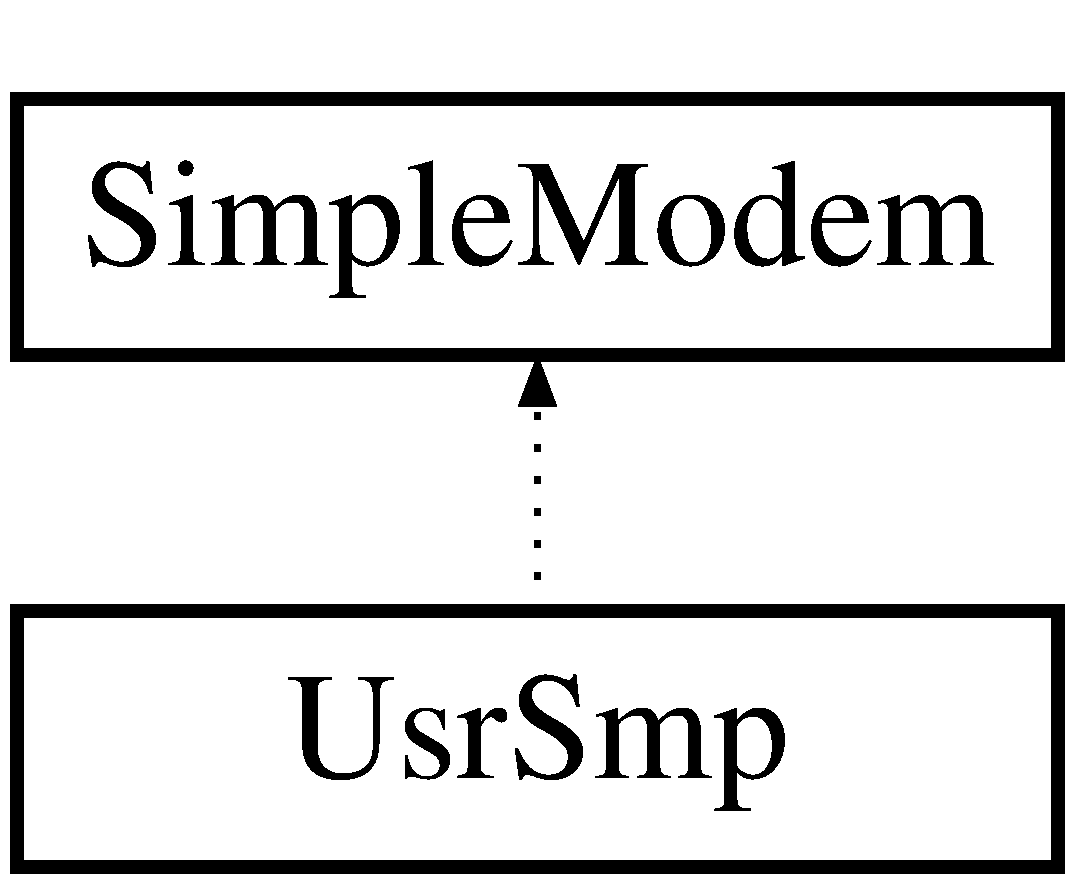
\includegraphics[height=2cm]{classUsrSmp}
\end{center}
\end{figure}
\subsection*{Public Member Functions}
\begin{CompactItemize}
\item 
{\bf Usr\-Smp} (QString interface=\char`\"{}/dev/tty\-S0\char`\"{}, QString baud=\char`\"{}115200\char`\"{})
\begin{CompactList}\small\item\em C'tor. \item\end{CompactList}\item 
{\bf $\sim$Usr\-Smp} ()
\begin{CompactList}\small\item\em D'tor. \item\end{CompactList}\item 
void {\bf Set\-Echo\-Off} ()
\begin{CompactList}\small\item\em Disable Echo (test). \item\end{CompactList}\item 
int {\bf Get\-Modem\-Type} ()\label{classUsrSmp_a3}

\begin{CompactList}\small\item\em Returns the modem type. \item\end{CompactList}\item 
int {\bf Set\-Stand\-Alone\-Mode} ()
\begin{CompactList}\small\item\em Sets stand alone mode for a USR modem. \item\end{CompactList}\item 
int {\bf Un\-Set\-Stand\-Alone\-Mode} ()
\begin{CompactList}\small\item\em Unsets stand alone mode for a USR modem. \item\end{CompactList}\item 
int {\bf Read\-Memory\-Info} ()
\begin{CompactList}\small\item\em Gets memory and message informations from the modem. \item\end{CompactList}\item 
QPtr\-List$<$ struct Message\-Info $>$ {\bf Get\-Msg\-Info} ()\label{classUsrSmp_a7}

\begin{CompactList}\small\item\em Returns information about all messages. \item\end{CompactList}\item 
Message\-Info {\bf Get\-Msg\-Info} (unsigned int index)\label{classUsrSmp_a8}

\begin{CompactList}\small\item\em Returns information about the specified Message. \item\end{CompactList}\item 
Memory\-Info {\bf Get\-Memory\-Info} ()\label{classUsrSmp_a9}

\begin{CompactList}\small\item\em Returns information about the memory. \item\end{CompactList}\item 
void {\bf Load\-Messages} ()\label{classUsrSmp_a10}

\begin{CompactList}\small\item\em This function load the stored messages to a temporary file. \item\end{CompactList}\item 
int {\bf Get\-Message} (int Message)
\begin{CompactList}\small\item\em This function gets the specified message from the temporary file. \item\end{CompactList}\item 
int {\bf Get\-Init\-Error} ()\label{classUsrSmp_a12}

\begin{CompactList}\small\item\em Returns the error wich happens in init. \item\end{CompactList}\end{CompactItemize}


\subsection{Detailed Description}
\begin{Desc}
\item[Author:]Alexander Wiedenbruch \end{Desc}




\subsection{Constructor \& Destructor Documentation}
\index{UsrSmp@{Usr\-Smp}!UsrSmp@{UsrSmp}}
\index{UsrSmp@{UsrSmp}!UsrSmp@{Usr\-Smp}}
\subsubsection{\setlength{\rightskip}{0pt plus 5cm}Usr\-Smp::Usr\-Smp (QString {\em interface} = {\tt \char`\"{}/dev/ttyS0\char`\"{}}, QString {\em baud} = {\tt \char`\"{}115200\char`\"{}})}\label{classUsrSmp_a0}


C'tor. 

Not much in here atm. \index{UsrSmp@{Usr\-Smp}!~UsrSmp@{$\sim$UsrSmp}}
\index{~UsrSmp@{$\sim$UsrSmp}!UsrSmp@{Usr\-Smp}}
\subsubsection{\setlength{\rightskip}{0pt plus 5cm}Usr\-Smp::$\sim${\bf Usr\-Smp} ()}\label{classUsrSmp_a1}


D'tor. 

Not much in here atm. 

\subsection{Member Function Documentation}
\index{UsrSmp@{Usr\-Smp}!GetMessage@{GetMessage}}
\index{GetMessage@{GetMessage}!UsrSmp@{Usr\-Smp}}
\subsubsection{\setlength{\rightskip}{0pt plus 5cm}int Usr\-Smp::Get\-Message (int {\em Message})}\label{classUsrSmp_a11}


This function gets the specified message from the temporary file. 

Partly (C) T. Uhlmann from usrmodem.cpp \index{UsrSmp@{Usr\-Smp}!ReadMemoryInfo@{ReadMemoryInfo}}
\index{ReadMemoryInfo@{ReadMemoryInfo}!UsrSmp@{Usr\-Smp}}
\subsubsection{\setlength{\rightskip}{0pt plus 5cm}int Usr\-Smp::Read\-Memory\-Info ()}\label{classUsrSmp_a6}


Gets memory and message informations from the modem. 

This function gets information about the memory first. After that it gets the information about all stored messages

Partly (C) T. Uhlmann from usrmodem.cpp \index{UsrSmp@{Usr\-Smp}!SetEchoOff@{SetEchoOff}}
\index{SetEchoOff@{SetEchoOff}!UsrSmp@{Usr\-Smp}}
\subsubsection{\setlength{\rightskip}{0pt plus 5cm}void Usr\-Smp::Set\-Echo\-Off ()}\label{classUsrSmp_a2}


Disable Echo (test). 

This function sends ATE0 to the modem. That command will disable the echoing \index{UsrSmp@{Usr\-Smp}!SetStandAloneMode@{SetStandAloneMode}}
\index{SetStandAloneMode@{SetStandAloneMode}!UsrSmp@{Usr\-Smp}}
\subsubsection{\setlength{\rightskip}{0pt plus 5cm}int Usr\-Smp::Set\-Stand\-Alone\-Mode ()}\label{classUsrSmp_a4}


Sets stand alone mode for a USR modem. 

Partly (C) T. Uhlmann from usrmodem.cpp \index{UsrSmp@{Usr\-Smp}!UnSetStandAloneMode@{UnSetStandAloneMode}}
\index{UnSetStandAloneMode@{UnSetStandAloneMode}!UsrSmp@{Usr\-Smp}}
\subsubsection{\setlength{\rightskip}{0pt plus 5cm}int Usr\-Smp::Un\-Set\-Stand\-Alone\-Mode ()}\label{classUsrSmp_a5}


Unsets stand alone mode for a USR modem. 

Partly (C) T. Uhlmann from usrmodem.cpp 

The documentation for this class was generated from the following files:\begin{CompactItemize}
\item 
usrsmp.h\item 
usrsmp.cpp\end{CompactItemize}
